\newpage
\selectlanguage{ukrainian}
%\renewcommand{\baselinestretch}{1.5}

\section{Вступ}



%\paragraph{} ~\\

\hspace*{8mm} Відокремлені хвилі, що зазвичай називаються солітонами, є обєктом інтенсивних досліджень в багатьох областях науки, таких як гідродинаміка, нелінійна оптика, фізика плазми так біологія. 

Історія вивчення солітонів бере початок в 1834 році, коли Джеймс Скотт Рассел помітив, що вал води в каналі розповсюджується без спотворень на протязі декількох кілометрів.

Однак властивості цих хвиль не були докладно досліджені до введення відповідних математичних моделей та розвитку методу оберненої задачі розсіяння. Термін "солітон" був введений у 1965 р., щоб наголосити на частинкоподібній природі відокремленних хвиль. 

В оптиці через наявність нелінійних ефектів, окрім явища дифракції наявне також явище самофокусування. Воно виникає внаслідок того, що в областях з більшою інтенсивністю світла показник заломлення вищій. 

Для деяких пучків світла самофокусування та розсіяння врівноважують одне одного, внаслідок чого відбувається так звана самолокалізація, або самоканалювання, і виникають стабільні структури (див. Рис. 1).

\begin{figure}
  \centering
  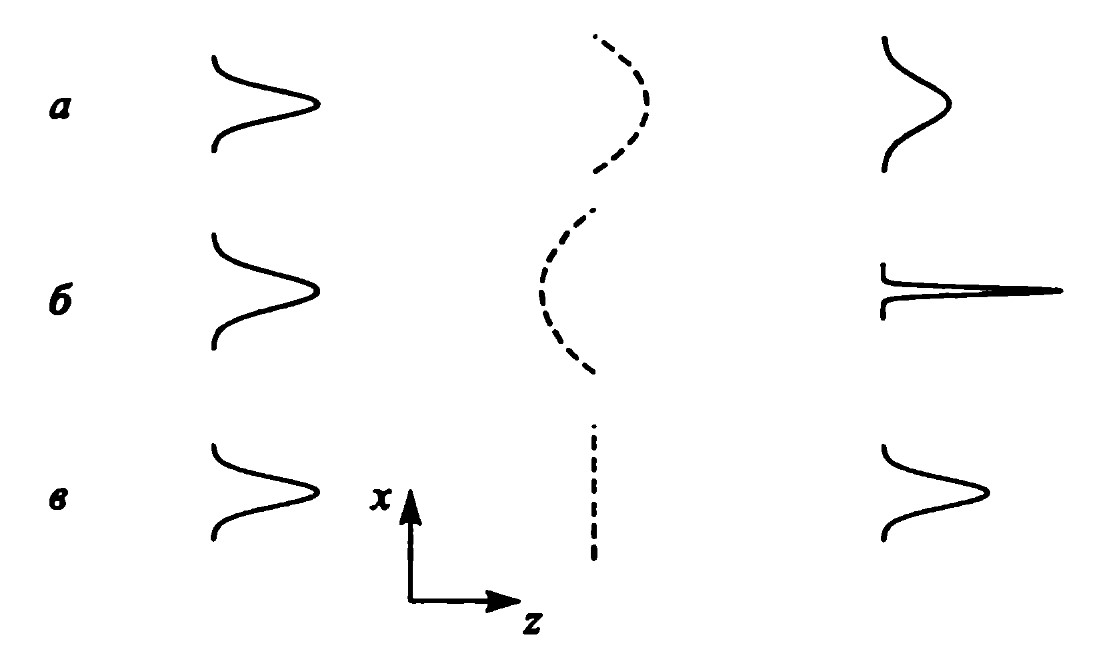
\includegraphics[width=300pt]{fig1}
  \caption{В першій колонці інтенсивність на вході, в другій - хвильовий фронт на виході, в третій - інтенсивність на виході для явищ (a) розсіяння, (б) самофокусування та (в) самолокалізації. \label{fig1}}
\end{figure} 

Ми розглядаємо два світлових вихори і будемо використовувати наступну систему рівнянь для опису еволюції світла в нелокальному середовищі з нелінійністю типу Керра:
\begin{equation}
   \begin{array}{1} {\displaystyle
       i\partial_z \Psi_n+\Delta_\perp\Psi_n +\theta\Psi_n=0,
       } \\*[9pt] {\displaystyle
\alpha^2\,\theta-\Delta_\perp\theta=|\Psi_1|^2+|\Psi_2|^2.
   }\end{array}
   \label{eq:NLS}
\end{equation}
де $\theta(x,y,z)$ - коефіцієнт заломлення світла, $\Psi_n$ - напруженість електричного поля зв'язаного з n-им світловим пучком, а n = 1,2.  



